\documentclass{../../../kin_math}

\lstset{basicstyle=\ttfamily, mathescape}

\header{Elijah Kin}{Homework 4}{AMSC660}
\headrule

\begin{document}

\begin{questions}
  \question Find an upper bound for the condition number for eigenvector $r_j$ of a non-symmetric matrix $A$ assuming that all its eigenvalues are distinct. In what case will this condition number be large?
  \begin{solution}
    As with the case when $A$ is symmetric, we start with the identity
    \begin{equation*}
      \dot{A}r_j + A\dot{r}_j = \dot{\lambda}_jr_j + \lambda_j\dot{r}_j
    \end{equation*}
    and expand the perturbation $\dot{r}_j$ in terms of the right eigenvectors $\{r_1, \dots, r_n\}$ to obtain
    \begin{equation*}
      \dot{A}r_j + A \sum_{i \neq j} m_{ji} r_i = \dot{\lambda}_jr_j + \lambda_j \sum_{i \neq j} m_{ji} r_i.
    \end{equation*}
    Further, multiplying on the left by $\ell_k$ yields
    \begin{equation*}
      \ell_k \dot{A}r_j + \ell_k A \sum_{i \neq j} m_{ji} r_i = \dot{\lambda}_j \ell_k r_j + \lambda_j \ell_k \sum_{i \neq j} m_{ji} r_i
    \end{equation*}
    and as a left eigenvector, $\ell_k A = \lambda_k \ell_k$, so
    \begin{equation*}
      \ell_k \dot{A}r_j + \lambda_k \ell_k \sum_{i \neq j} m_{ji} r_i = \dot{\lambda}_j \ell_k r_j + \lambda_j \ell_k \sum_{i \neq j} m_{ji} r_i
    \end{equation*}
    Then due to the fact that $L = R^{-1}$, so $\ell_i r_j = \delta_{ij}$ and by assuming $k \neq j$,
    \begin{equation*}
      \ell_k \dot{A}r_j + \lambda_k m_{jk} = \lambda_j m_{jk}
    \end{equation*}
    and hence solving for $m_{jk}$ yields
    \begin{equation*}
      m_{jk} = \frac{\ell_k \dot{A}r_j}{\lambda_j - \lambda_k}.
    \end{equation*}
    We can then write
    \begin{equation*}
      \dot{r}_j = \sum_{k \neq j} m_{jk} r_k = \sum_{k \neq j} \frac{\ell_k \dot{A}r_j}{\lambda_j - \lambda_k} r_k
    \end{equation*}
    and so multiplying by $\Delta t$ and applying the identities $\Delta r_j = \dot{r}_j \Delta t + O(\lVert \Delta A \rVert^2)$ and $\Delta A = \dot{A} \Delta t + O(\lVert \Delta A \rVert^2)$,
    \begin{equation*}
      \Delta r_j = \sum_{k \neq j} \frac{\ell_k \Delta A r_j}{\lambda_j - \lambda_k} r_k + O(\lVert \Delta A \rVert^2).
    \end{equation*}
    Now ignoring the $O(\lVert \Delta A \rVert^2)$ term and using the known bound for $|\ell_k \Delta A r_j|$,
    \begin{multline*}
      \lVert \Delta r_j \rVert = \left\lVert \sum_{k \neq j} \frac{\ell_k \Delta A r_j}{\lambda_j - \lambda_k} r_k \right\rVert \leq \sum_{k \neq j} \left\lVert \frac{\ell_k \Delta A r_j}{\lambda_j - \lambda_k} r_k \right\rVert = \sum_{k \neq j} \frac{|\ell_k \Delta A r_j|}{|\lambda_j - \lambda_k|} \lVert r_k \rVert \\
      \leq \sum_{k \neq j} \frac{\lVert \ell_k \rVert \lVert \Delta A \rVert \lVert r_j \rVert}{|\lambda_j - \lambda_k|} \lVert r_k \rVert = \lVert \Delta A \rVert \sum_{k \neq j} \frac{\lVert \ell_k \rVert \lVert r_k \rVert \lVert r_j \rVert}{|\lambda_j - \lambda_k|}.
    \end{multline*}
    Hence,
    \begin{multline*}
      \kappa(r_j; A) = \lim_{\epsilon \to 0} \max_{\lVert \Delta A \rVert = \epsilon} \frac{\lVert \Delta r_j \rVert \lVert A \rVert}{\lVert r_j \rVert \lVert \Delta A \rVert} \leq \frac{\lVert \Delta A \rVert \sum_{k \neq j} \frac{\lVert \ell_k \rVert \lVert r_k \rVert \lVert r_j \rVert}{|\lambda_j - \lambda_k|} \lVert A \rVert}{\lVert r_j \rVert \lVert \Delta A \rVert} \\
      = \sum_{k \neq j} \frac{\lVert \ell_k \rVert \lVert r_k \rVert}{|\lambda_j - \lambda_k|} \lVert A \rVert = \lVert A \rVert \sum_{k \neq j} (\lambda_j - \lambda_k)^{-1} \lVert \ell_k \rVert \lVert r_k \rVert
    \end{multline*}
    which we can further simplify via the bound $\lVert \ell_k \rVert \lVert r_k \rVert \leq \lVert R^{-1} \rVert \lVert R \rVert$ to see
    \begin{equation*}
      \kappa(r_j; A) \leq \lVert A \rVert \lVert R^{-1} \rVert \lVert R \rVert \sum_{k \neq j} (\lambda_j - \lambda_k)^{-1}
    \end{equation*}
    This bound shows that the condition number could be large if there is an eigenvalue close to $\lambda_j$, or if the matrix of eigenvectors is ill-conditioned, or if the largest singular value of $A$ is very large (and hence $\lVert A \rVert$ is large).
  \end{solution}

  \question Let $A$ be an $n \times n$ matrix. The Rayleigh quotient $Q(x)$ is the following function defined on all $x \in \mathbb{R}^n$:
  \begin{equation*}
    Q(x) \coloneqq \frac{x^\top Ax}{x^\top x}.
  \end{equation*}
  \begin{enumerate}
    \item Let $A$ be symmetric. Prove that $\nabla Q(x) = 0$ if and only if $x$ is an eigenvector of $A$.
    \begin{solution}
      By the quotient rule, we have that
      \begin{multline*}
        \frac{\partial Q}{\partial x_i} = \frac{(x^\top x) \frac{\partial}{\partial x_i} [x^\top A x] - (x^\top A x) \frac{\partial}{\partial x_i} [x^\top x]}{(x^\top x)^2} = \frac{\frac{\partial}{\partial x_i} [x^\top A x]}{x^\top x} - \frac{(x^\top A x) \frac{\partial}{\partial x_i} [x^\top x]}{(x^\top x)^2} \\
        = \frac{\frac{\partial}{\partial x_i} [x^\top A x]}{x^\top x} - \frac{Q(x) \frac{\partial}{\partial x_i} [x^\top x]}{x^\top x} = \frac{1}{x^\top x} \left(\frac{\partial}{\partial x_i}[x^\top A x] - Q(x) \frac{\partial}{\partial x_i}[x^\top x]\right).
      \end{multline*}
      Then towards simplifying this expression further, note that
      \begin{equation*}
        \frac{\partial}{\partial x_i}[x^\top x] = \frac{\partial}{\partial x_i} \sum_{j = 1}^n x_j^2 = \sum_{j = 1}^n \frac{\partial}{\partial x_i} x_j^2 = \frac{\partial}{\partial x_i} x_i^2 = 2x_i
      \end{equation*}
      and also that by the product rule,
      \begin{multline*}
        \frac{\partial}{\partial x_i}[x^\top A x] = \frac{\partial}{\partial x_i} \sum_{j = 1}^n x_j (Ax)_j = \sum_{j = 1}^n \frac{\partial}{\partial x_i} [x_j (Ax)_j] = \sum_{j = 1}^n (Ax)_j \frac{\partial}{\partial x_i} [x_j] + x_j \frac{\partial}{\partial x_i} [(Ax)_j] \\
        = \sum_{j = 1}^n (Ax)_j \frac{\partial}{\partial x_i} [x_j] + \sum_{j = 1}^n x_j \frac{\partial}{\partial x_i} [(Ax)_j] = (Ax)_i + \sum_{j = 1}^n x_j \frac{\partial}{\partial x_i} \left[\sum_{k = 1}^n a_{jk} x_k \right] \\
        = (Ax)_i + \sum_{j = 1}^n x_j \sum_{k = 1}^n a_{jk} \frac{\partial}{\partial x_i} x_k = (Ax)_i + \sum_{j = 1}^n a_{ji} x_j = (Ax)_i + (A^\top x)_i.
      \end{multline*}
      Hence, without yet assuming $A$ is symmetric,
      \begin{equation*}
        \frac{\partial Q}{\partial x_i} = \frac{1}{x^\top x} \left((Ax)_i + (A^\top x)_i - 2 Q(x) x_i\right)
      \end{equation*}
      and so
      \begin{equation}
        \label{eq:grad}
        \nabla Q(x) = \frac{1}{x^\top x} \left(Ax + A^\top x - 2 Q(x) x\right) = \frac{1}{x^\top x} \left((A + A^\top)x - 2 Q(x) x\right).
      \end{equation}
      Then if $A$ is symmetric, meaning that $A + A^\top = 2A$,
      \begin{equation*}
        \nabla Q(x) = \frac{1}{x^\top x} \left(2Ax - 2 Q(x) x\right) = \frac{2}{x^\top x} \left(Ax - Q(x) x\right).
      \end{equation*}
      Now if $\nabla Q(x) = 0$ then it must be that $Ax - Q(x)x = 0$, and so
      \begin{equation*}
        Ax = Q(x)x
      \end{equation*}
      meaning $x$ is an eigenvector of $A$. Similarly, if $x$ is an eigenvector of $A$ corresponding to $\lambda$,
      \begin{equation*}
        Q(x) = \frac{x^\top A x}{x^\top x} = \frac{x^\top \lambda x}{x^\top x} = \lambda \frac{x^\top x}{x^\top x} = \lambda
      \end{equation*}
      and so $\nabla Q(x) = 0$. Hence, $\nabla Q(x) = 0$ if and only if $x$ is an eigenvector of $A$.
    \end{solution}
    \item Let $A$ be asymmetric. What are the vectors $x$ at which $\nabla Q = 0$?
    \begin{solution}
      Recall from (\ref{eq:grad}) that
      \begin{equation*}
        \nabla Q(x) = \frac{1}{x^\top x} \left((A + A^\top)x - 2 Q(x) x\right)
      \end{equation*}
      hence if $\nabla Q(x) = 0$ then $(A + A^\top)x - 2Q(x) x = 0$ and so
      \begin{equation*}
        (A + A^\top)x = 2Q(x)x,
      \end{equation*}
      meaning $\nabla Q(x) = 0$ when $x$ is an eigenvector of $A + A^\top$.
    \end{solution}
  \end{enumerate}

  \question Consider the Rayleigh Quotient Iteration, a very efficient algorithm for finding an eigenpair of a given matrix
  \begin{lstlisting}
    Input: $x_0 \neq 0$ is the initial guess for an eigenvector
    $v = x_0 / \lVert x_0 \rVert$
    for k = 0, 1, 2, $\dots$
      $\mu_k = v^\top A v$
      Solve $(A - \mu_k I)w = v$ for $w$
      $v = w / \lVert w \rVert$.
    end for
  \end{lstlisting}
  Here is a Matlab program implementing the Rayleigh Quotient Iteration for finding an eigenpair of a random $n \times n$ symmetric matrix starting from a random initial guess:
  \begin{lstlisting}
    function RayleighQuotient()
    n = 100;
    A = rand(n);
    A = A' + A;
    v = rand(n, 1);
    v = v / norm(v);
    k = 1;
    mu(k) = v' * A * v;
    tol = 1e-12;
    I = eye(n);
    res = abs(norm(A * v - mu(k) * v) / mu(k));
    fprintf('k = %d: lam = %d\tres = %d\n', k, mu(k), res);
    while res > tol
      w = (A - mu(k) * I) \ v;
      k = k + 1;
      v = w / norm(w);
      mu(k) = v' * A * v;
      res = abs(norm(A * v - mu(k) * v) / mu(k));
      fprintf('k = %d: lam = %d\tres = %d\n', k mu(k), res);
    end
    end
  \end{lstlisting}
  \begin{enumerate}
    \item Let $A$ be a symmetric matrix with all distinct eigenvalues. Let $\mu$ be not an eigenvalue of $A$. Show that if $(\lambda, v)$ is an eigenpair of $A$ then $((\lambda - \mu)^{-1}, v)$ is an eigenpair of $(A - \mu I)^{-1}$.
    \begin{solution}
      If $(\lambda, v)$ is an eigenpair of $A$, then $Av = \lambda v$. We want to show that
      \begin{equation*}
        (A - \mu I)^{-1} v = (\lambda - \mu)^{-1} v,
      \end{equation*}
      which by left multiplying both sides by $(A - \mu I)$ is equivalent to
      \begin{multline*}
        v = (\lambda - \mu)^{-1} (A - \mu I)v = (\lambda - \mu)^{-1} (Av - \mu Iv) \\
        = (\lambda - \mu)^{-1} (\lambda v - \mu v) = (\lambda - \mu)^{-1} (\lambda - \mu) v = v
      \end{multline*}
      which is clearly true. Hence, $(A - \mu I)^{-1} v = (\lambda - \mu)^{-1} v$ is also true, so $((\lambda - \mu)^{-1}, v)$ is an eigenpair of $(A - \mu I)^{-1}$.
    \end{solution}
    \item The Rayleigh Quotient iteration involves solving the system $(A - \mu_k I) w = v$ for $w$. The matrix $(A - \mu_k I)$ is close to singular. Nevertheless, this problem is well-conditioned (in exact arithmetic). Explain this phenomenon. Proceed as follows. Without the loss of generality assume that $v$ is an approximation for the eigenvector $v_1$ of $A$, and $\mu$ is an approximation to the corresponding eigenvalue $\lambda_1$. Let $\lVert v \rVert = 1$. Write $v$ as
    \begin{equation*}
      v = \left(1- \sum_{i = 2}^n \delta_i^2\right)^{1 / 2} v_1 + \sum_{i = 2}^n \delta_i v_i,
    \end{equation*}
    where $\delta_i$, $i = 2, \dots, n$, are small. Show that the condition number $\kappa((A - \mu I)^{-1}, v)$ (see page 88 in \href{https://math.nyu.edu/~shelley/Classes/SciComp/BindelGoodman.pdf}{Bindel and Goodman, Principles of scientific computing}) is approximately $(1 - \sum_{i = 2}^n \delta_i^2)^{-1 / 2}$ which is close to 1 provided that $\delta_i$ are small.
    \begin{solution}
      From page 88 of Bindel, we have that the condition number for solving the linear system $Au = b$ is given by
      \begin{equation*}
        \kappa(A^{-1}, b) = \lVert A^{-1} \rVert \frac{\lVert b \rVert}{\lVert A^{-1} b \rVert}
      \end{equation*}
      and so given the system $(A - \mu_k I) w = v$,
      \begin{equation*}
        \kappa((A - \mu I)^{-1}, v) = \lVert (A - \mu I)^{-1} \rVert \frac{\lVert v \rVert}{\lVert (A - \mu I)^{-1} v \rVert}
      \end{equation*}
      and so assuming $\lVert v \rVert = 1$,
      \begin{equation}
        \label{eq:cond}
        \kappa((A - \mu I)^{-1}, v) = \lVert (A - \mu I)^{-1} \rVert \frac{1}{\lVert (A - \mu I)^{-1} v \rVert}.
      \end{equation}
      By part (a), the eigenvalues of $(A - \mu I)^{-1}$ are $(\lambda_i - \mu)^{-1}$. Further, since $A$ is symmetric then so $(A - \mu I)^{-1}$, and so by (1) of Theorem 3, its singular values are
      \begin{equation*}
        |(\lambda_i - \mu)^{-1}| = \frac{1}{|\lambda_i - \mu|}
      \end{equation*}
      the largest of which will be attained by $i = 1$, since $\mu$ approximates $\lambda_1$.
      Hence, by (5) of Theorem 3,
      \begin{equation*}
        \lVert (A - \mu I)^{-1} \rVert = \frac{1}{|\lambda_1 - \mu|},
      \end{equation*}
      and so substituting into (\ref{eq:cond}), we obtain
      \begin{equation*}
        \kappa((A - \mu I)^{-1}, v) = \frac{1}{|\lambda_1 - \mu|} \frac{1}{\lVert (A - \mu I)^{-1} v \rVert}.
      \end{equation*}
      Then writing
      \begin{equation*}
        v = \left(1- \sum_{i = 2}^n \delta_i^2\right)^{1 / 2} v_1 + \sum_{i = 2}^n \delta_i v_i
      \end{equation*}
      and noting from part (a) that $(A - \mu I)^{-1} v_i = (\lambda_i - \mu)^{-1} v_i$, we have
      \begin{multline*}
        \lVert (A - \mu I)^{-1} v \rVert = \left\lVert \left(1- \sum_{i = 2}^n \delta_i^2\right)^{1 / 2} (A - \mu I)^{-1} v_1 + \sum_{i = 2}^n \delta_i (A - \mu I)^{-1} v_i \right\rVert \\
        = \left\lVert \left(1- \sum_{i = 2}^n \delta_i^2\right)^{1 / 2} (\lambda_1 - \mu)^{-1} v_1 + \sum_{i = 2}^n \delta_i (\lambda_i - \mu)^{-1} v_i \right\rVert.
      \end{multline*}
      Hence, since the eigenvalues are distinct, the eigenvectors form an orthonormal basis,
      \begin{multline*}
        \kappa((A - \mu I)^{-1}, v) = \frac{1}{|\lambda_1 - \mu|} \frac{1}{\lVert (A - \mu I)^{-1} v \rVert} \\
        = \left\lVert \left(1- \sum_{i = 2}^n \delta_i^2\right)^{1 / 2} v_1 + \sum_{i = 2}^n \delta_i \frac{\lambda_1 - \mu}{\lambda_i - \mu} v_i \right\rVert^{-1} \\
        = \left(\left(1- \sum_{i = 2}^n \delta_i^2\right) + \sum_{i = 2}^n \left(\delta_i \frac{\lambda_1 - \mu}{\lambda_i - \mu}\right)^2 \right)^{-1 / 2} \\
        = \left(1- \sum_{i = 2}^n \delta_i^2 \left( 1 - \left(\frac{\lambda_1 - \mu}{\lambda_i - \mu}\right)^2\right) \right)^{-1 / 2}
      \end{multline*}
      and so from the fact that $\mu \approx \lambda_1$, we find that
      \begin{equation*}
        \kappa((A - \mu I)^{-1}, v) \approx \left(1- \sum_{i = 2}^n \delta_i^2\right)^{-1 / 2}.
      \end{equation*}
    \end{solution}
    \item It is known that the Rayleigh Quotient iteration converges cubically, which means that the error $e_k \coloneqq |\lambda - \mu_k|$ decays with $k$ so that the limit
    \begin{equation*}
      \lim_{k \to \infty} \frac{e_{k + 1}}{e_k^3} = C \in (0, \infty).
    \end{equation*}
    This means that the number of correct digits in $\mu_k$ triples with each iteration. Try to check this fact experimentally and report your findings. Proceed as follows. Run the program. Treat the final $\mu_k$ as the exact eigenvalue. Define $e_j \coloneqq |\mu_j - \mu_k|$ for $j = 1, \dots, k - 1$. Etc. Pick several values of $n$ and make several runs for each $n$. Note that you might not observe the cubic rate of convergence due to too few iterations and floating point arithmetic.
    \begin{solution}
      We observe cubic convergence for $n \in \{10, 50, 100, 500, 1000\}$ from the code \href{https://github.com/elijahkin/school/blob/main/umd/amsc660/hw4.ipynb}{here}. In particular, in each case plotting the ratio
      \begin{equation*}
        \frac{e_{j + 1}}{e_j^3}
      \end{equation*}
      as a function of the iteration number $j$, the ratio appears to level out given the three available points for each value of $n$. We show the plot for $n = 500$ below.
      \begin{center}
        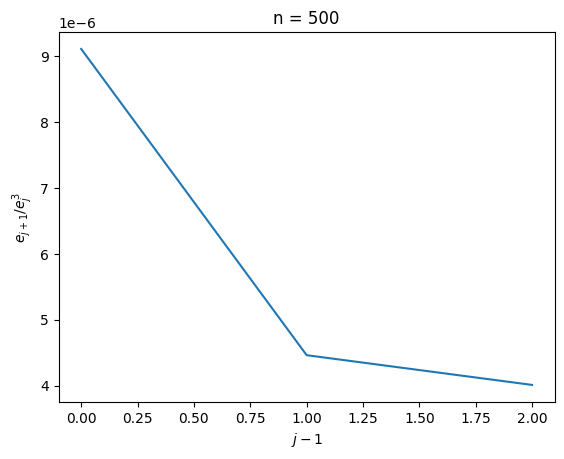
\includegraphics[scale=0.7]{cubic500.png}
      \end{center}
    \end{solution}
  \end{enumerate}
\end{questions}

\end{document}
